\section{Methodology \& Implementation} 


\begin{frame}[label=timeline, shrink]{Project Timeline: From Data to Prediction}

\begin{center}
\centerresizebox{
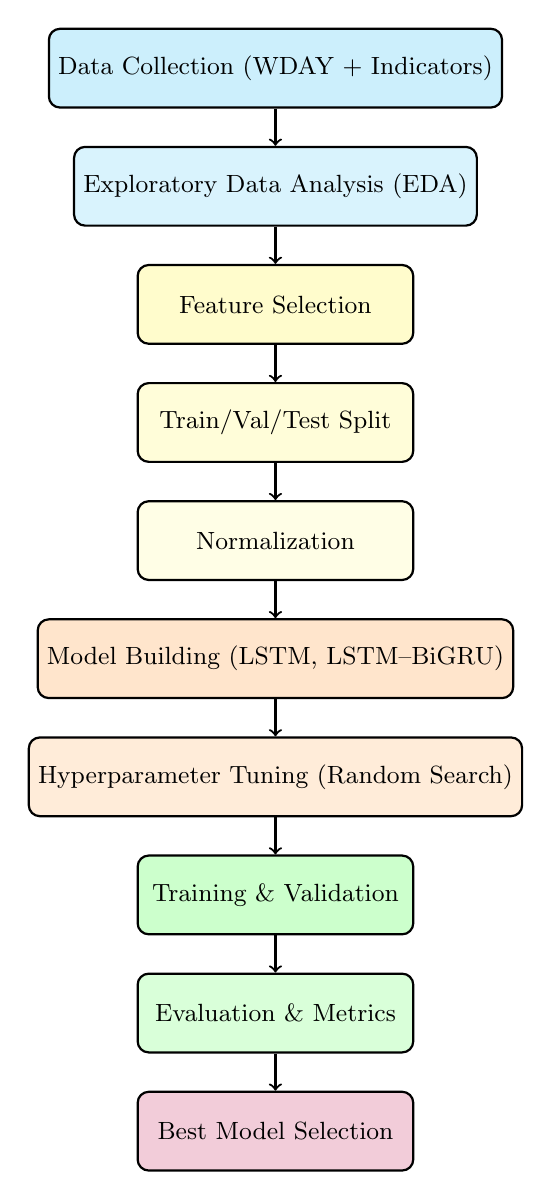
\begin{tikzpicture}[node distance=1.5cm, every node/.style={draw, rectangle, rounded corners, minimum width=3.5cm, minimum height=1cm, font=\small, align=center}, every path/.style={draw, thick, ->}]

% Nodes
\node[fill=cyan!20]  (start) {Data Collection (WDAY + Indicators)};
\node[fill=cyan!15] (eda) [below of=start] {Exploratory Data Analysis (EDA)};
\node[fill=yellow!20] (feature) [below of=eda] {Feature Selection};
\node[fill=yellow!15] (split) [below of=feature] {Train/Val/Test Split};
\node[fill=yellow!10] (normalization) [below of=split] {Normalization};
\node[fill=orange!20] (build) [below of=normalization] {Model Building (LSTM, LSTM–BiGRU)};
\node[fill=orange!15] (tuning) [below of=build] {Hyperparameter Tuning (Random Search)};
\node[fill=green!20] (train) [below of=tuning] {Training \& Validation};
\node[fill=green!15] (evaluation) [below of=train] {Evaluation \& Metrics};
\node[fill=purple!20] (end) [below of=evaluation] {Best Model Selection};

% Arrows
\draw (start) -- (eda);
\draw (eda) -- (feature);
\draw (feature) -- (split);
\draw (split) -- (normalization);
\draw (normalization) -- (build);
\draw (build) -- (tuning);
\draw (tuning) -- (train);
\draw (train) -- (evaluation);
\draw (evaluation) -- (end);

\end{tikzpicture}
}
\end{center}

\note{
This diagram outlines the full deep learning pipeline used to predict Workday’s stock price.

We begin with data collection, which includes WDAY historical prices and technical indicators like moving averages and RSI. Next, we perform exploratory data analysis to understand trends, patterns, and data quality.

Feature selection reduces noise by retaining only the most relevant inputs. The dataset is then split chronologically into training, validation, and test sets, and normalized to ensure stable input ranges for LSTM models.

Model building involves creating both LSTM and LSTM–BiGRU architectures, which are capable of capturing temporal dependencies. We tune hyperparameters like layer size, learning rate, and dropout using random search to optimize performance.

The best model is trained and validated, and evaluated on the test set using metrics like MAE and RMSE. Finally, the most robust and generalizable model is selected for analysis.

This structured process ensures the models are both well-tuned and realistically tested under conditions of volatility and limited data.
}
\end{frame}

\begin{frame}[label=datastructure,shrink]{Dataset Overview: Features and Indicators}
\begin{table}
\centering
\caption{Categories of Features in the WDAY Dataset}
\label{tab:datasetstructure}
\renewcommand{\arraystretch}{1.7} 
\begin{tabular}{p{2cm}p{12.5cm}}
\hline
\textbf{Category} & \textbf{Description} \\
\hline\hline
\textbf{Pricing} & Includes daily Open, High, Low, Close, and Volume (OHLCV) 
values, serving as the \alert{foundation for tracking stock performance}. \\
\textbf{Trend} & Measure the overall market direction, 
\alert{helping to identify uptrends, downtrends}, or sideways movements. \textit{Example: Moving Average Convergence Divergence (MACD)}. \\
\textbf{Momentum} & Evaluate the \alert{speed and strength of price movements},
providing insights into potential trend reversals and overbought/oversold 
conditions. \textit{Example: Relative Strength Index (RSI)}. \\
\textbf{Volatility} & Assess market risk and \alert{price fluctuations}, identifying 
potential breakouts and periods of stability. {\textit{Example: Bollinger Bands Width}.} \\
\textbf{Volume} & Analyze trading activity to confirm price trends and \alert{detect accumulation (buying) or distribution (selling) behavior}. \textit{Example: On-Balance Volume (OBV)}. \\
\hline
\end{tabular}
\end{table}

\note{
The dataset is structured around five major feature categories.
Pricing Data (OHLCV) forms the base, while Trend, Momentum, Volatility, and Volume indicators enrich the inputs.
These indicators offer critical signals about market behavior, improving the model's ability to forecast stock price movements.
Using multiple indicator types ensures the model captures various dimensions of stock performance, not just raw prices.
}
\end{frame}

\begin{frame}[label=datasetsplit, shrink]{Dataset Split Strategy}

\small

\begin{block}{Why Time-Based Splitting?}
\begin{itemize}
    \item Time-series data must maintain chronological order to avoid data leakage.
    \item Ensures that the model only uses \textbf{past} information to predict the \textbf{future}.
    \item Aligns with best practices in financial forecasting research~\parencite{chang2024StockPrediction, guo2024LSTMStock}.
\end{itemize}
\end{block}

\vspace{0.5em}
{\footnotesize
\begin{equation}
\label{eq:dataset_split_dates}
\underbrace{X_{\text{2014-01-02}}, \dots, X_{\text{2021-11-08}}}_{\text{Training Data (75\%)}} 
\quad
\underbrace{X_{\text{2021-11-09}}, \dots, X_{\text{2023-07-20}}}_{\text{Validation Data (15\%)}} 
\quad
\underbrace{X_{\text{2023-07-21}}, \dots, X_{\text{2025-03-28}}}_{\text{Test Data (15\%)}} 
\end{equation}
}
\note{
In financial forecasting, preserving the temporal structure is crucial.

We split the dataset chronologically:
\begin{itemize}
    \item 75\% for training — covering over 7 years of historical patterns.
    \item 15\% for validation — tuning hyperparameters.
    \item 15\% for testing — strictly future, unseen data from volatile periods.
\end{itemize}
The chronological split avoids any future data leakage into training and reflects real-world stock prediction challenges.
}
\end{frame}

\begin{frame}[label=lstm_architecture]{Model Architecture -- Layered LSTM}

\begin{columns}[c] % center vertically aligned
    \begin{column}{0.7\textwidth}
        \begin{block}{Overview}
            \begin{itemize}
                \item Two stacked LSTM layers to capture long-term sequential patterns.
                \item Dropout layers after each LSTM to prevent overfitting.
                \item Dense output layer to predict the next day's closing price.
                \item Simple yet powerful model for financial time-series forecasting.
            \end{itemize}
        \end{block}
    \end{column}
    
    \begin{column}{0.28\textwidth}
        \centering
        \resizebox{0.7\textwidth}{!}{
        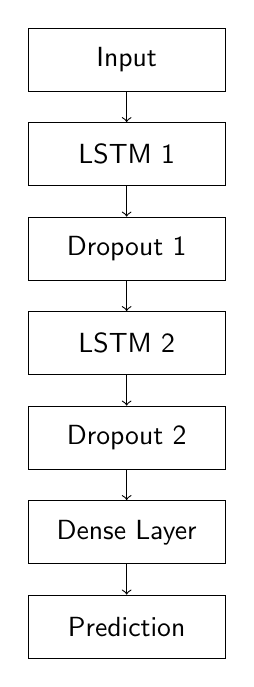
\begin{tikzpicture}[node distance=1.2cm, every node/.style={draw, minimum width=2.5cm, minimum height=0.8cm, font=\sffamily, align=center}]
            \node(input) {Input};
            \node[below of=input] (lstm1) {LSTM 1};
            \node[below of=lstm1] (drop1) {Dropout 1};
            \node[below of=drop1] (lstm2) {LSTM 2};
            \node[below of=lstm2] (drop2) {Dropout 2};
            \node[below of=drop2] (dense) {Dense Layer};
            \node[below of=dense] (output) {Prediction};
            \draw[->] (input) -- (lstm1);
            \draw[->] (lstm1) -- (drop1);
            \draw[->] (drop1) -- (lstm2);
            \draw[->] (lstm2) -- (drop2);
            \draw[->] (drop2) -- (dense);
            \draw[->] (dense) -- (output);
        \end{tikzpicture}
        }
    \end{column}
\end{columns}

\note{
The LSTM architecture uses two LSTM layers to model long-term temporal dependencies,
followed by dropout layers to regularize the model and prevent overfitting.
Finally, a Dense layer maps the learned representations into a next-day price prediction.
This simple but robust design is commonly used in stock forecasting tasks.

Just as adding exponents or higher-order terms makes a mathematical function more flexible and expressive, stacking LSTM or BiGRU layers enhances the model’s ability to learn complex, long-term patterns in sequential stock price data.
}
\end{frame}


\begin{frame}[label=lstmbigru_architecture]{Model Architecture -- Hybrid LSTM-BiGRU}

\begin{columns}[c]
    \begin{column}{0.7\textwidth}
        \begin{block}{Overview}
            \begin{itemize}
                \item BiGRU layer captures both past and future dependencies.
                \item Followed by 3 stacked LSTM layers for sequence refinement.
                \item Dropout layers prevent overfitting at each stage.
                \item Dense layer outputs the next-day stock price.
            \end{itemize}
        \end{block}
    \end{column}
    
    \begin{column}{0.28\textwidth}
        \resizebox{0.45\textwidth}{!}{
        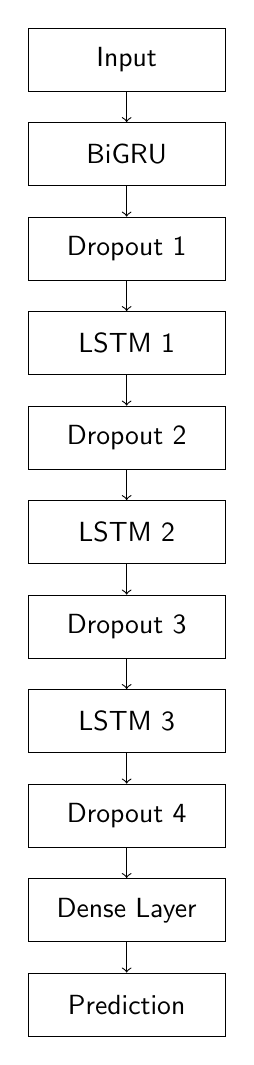
\begin{tikzpicture}[node distance=1.2cm, every node/.style={draw, minimum width=2.5cm, minimum height=0.8cm, font=\sffamily, align=center}]
            \node(input) {Input};
            \node[below of=input] (bigru) {BiGRU};
            \node[below of=bigru] (drop1) {Dropout 1};
            \node[below of=drop1] (lstm1) {LSTM 1};
            \node[below of=lstm1] (drop2) {Dropout 2};
            \node[below of=drop2] (lstm2) {LSTM 2};
            \node[below of=lstm2] (drop3) {Dropout 3};
            \node[below of=drop3] (lstm3) {LSTM 3};
            \node[below of=lstm3] (drop4) {Dropout 4};
            \node[below of=drop4] (dense) {Dense Layer};
            \node[below of=dense] (output) {Prediction};
            \draw[->] (input) -- (bigru);
            \draw[->] (bigru) -- (drop1);
            \draw[->] (drop1) -- (lstm1);
            \draw[->] (lstm1) -- (drop2);
            \draw[->] (drop2) -- (lstm2);
            \draw[->] (lstm2) -- (drop3);
            \draw[->] (drop3) -- (lstm3);
            \draw[->] (lstm3) -- (drop4);
            \draw[->] (drop4) -- (dense);
            \draw[->] (dense) -- (output);
        \end{tikzpicture}
        }
    \end{column}
\end{columns}

\note{
The LSTM-BiGRU hybrid architecture first uses a BiGRU to capture sequential information from both directions.
Then, three LSTM layers refine the learned patterns, allowing the model to better detect future stock trends.
Dropouts help prevent overfitting, while the final Dense layer generates the next-day price prediction.
}
\end{frame}

\begin{frame}[label=final_models]{Final Model Architectures and Parameters}

\begin{columns}[c]
\column{0.48\textwidth}
\textbf{LSTM Model:}
\vspace{0.3em}
\begin{table}[H]
\centering
\resizebox{\linewidth}{!}{
\begin{tabular}{lp{2.8cm}}
\hline
\textbf{Parameter} & \textbf{Value} \\
\hline\hline
Sequence Length & 30 \\
Hidden Units & LSTM$_1$: 128, LSTM$_2$: 32 \\
Dropout Rates & 0.01 after each LSTM layer \\
Dense Layer & 32 units \\
Learning Rate & 0.001 \\
Total Parameters & 292,421 \\
Trainable Parameters & 97,473 \\
\hline
\end{tabular}
}
\end{table}

\column{0.48\textwidth}
\textbf{LSTM-BiGRU Model:}
\vspace{0.3em}
\begin{table}[H]
\centering
\resizebox{\linewidth}{!}{
\begin{tabular}{lp{2.8cm}}
\hline
\textbf{Parameter} & \textbf{Value} \\
\hline\hline
Sequence Length & 30 \\
Hidden Units & BiGRU: 64, LSTM$_1$: 64, LSTM$_2$: 32, LSTM$_3$: 16 \\
Dropout Rates & BiGRU: 0.01, LSTM$_1$: 0.3, LSTM$_2$: 0.2, LSTM$_3$: 0.01
\\
Dense Layer & 16 units \\
Learning Rate & 0.001 \\
Total Parameters & 293,669 \\
Trainable Parameters & 97,889 \\
\hline
\end{tabular}
}
\end{table}

\end{columns}

\note{
This slide compares the architectural details of the LSTM and LSTM–BiGRU models used in our experiments.

Both models use a sequence length of 30, allowing them to learn from 30 prior time steps. The LSTM model features two stacked layers with 128 and 32 hidden units, and minimal regularization through a uniform dropout rate of 0.01. Its dense output layer has 32 units.

In contrast, the LSTM–BiGRU model incorporates a BiGRU layer with 64 units followed by three LSTM layers with decreasing units (64, 32, 16). This deeper structure is complemented by more aggressive and layer-specific dropout: 0.3 and 0.2 in the early LSTM layers, which helps mitigate overfitting.

Interestingly, both models maintain comparable complexity, with the LSTM–BiGRU model having just slightly more parameters—less than a 1\% increase. This means the performance gains from the hybrid model come from its structure, not its size.

This comparison supports the hypothesis that hybrid and deeper recurrent architectures may be better suited for capturing the volatility and weak signals in mid-cap stock data like Workday.

The second model outperforms the first because its deeper, hybrid architecture is better suited to capturing the non-linear and context-dependent patterns often found in volatile mid-cap stock data like Workday.
}
\end{frame}

\begin{frame}[shrink]{Performance - Training and Validation Loss Comparison}
\centering
\resizebox{1.3\linewidth}{!}{%
\begin{tabular}{m{2cm}m{10cm}}
    \textbf{LSTM} & \includegraphics[width=0.7\textwidth]{img/main/lstm_loss.png} \\
    \textbf{LSTM-BiGRU} & \includegraphics[width=0.7\textwidth]{img/main/bigru_loss.png} \\
\end{tabular}
}
\note{
Loss - Shows convergence during training (e.g., MSE or custom loss). Always 
start with Loss curves.1
Both models converge smoothly. However, the LSTM-BiGRU achieves slightly lower 
validation loss earlier, suggesting faster convergence and slightly better 
generalization.
}
\end{frame}
